\documentclass[10pt,twocolumn]{article}

% Builds with plain pdflatex (no conference style files needed).
\usepackage[margin=0.85in]{geometry}
\usepackage{booktabs}
\usepackage{multirow}
\usepackage{amsmath}
\usepackage{amssymb}
\usepackage{amstext}
\usepackage{graphicx}
\graphicspath{{figures/}}
\usepackage[hidelinks]{hyperref}
\usepackage{caption}
\captionsetup{font=small}

\newcommand{\uu}[1]{\,\textsf{#1}}

\title{\vspace{-2em}\bfseries OS Noise for Agentic AI:\\
A Kernel-Trace Study of How Container Resource Limits\\
Slow Down and Break AI Coding Agents}

\author{Yuvraj Sehgal \quad Naser Ezzati-Jivan\\
\small Department of Computer Science \quad (draft --- \today)}
\date{}

\begin{document}
\maketitle

\begin{abstract}
When a coding agent is slow, the usual diagnosis is the language model. But
agents run inside containers, and containers come with resource limits (a
fractional CPU, a memory ceiling, an I/O budget) set by whatever platform
runs them. We ask how much of an agent's wall-clock time these limits
silently take. We answer with kernel tracing (LTTng) on two production
agents, \emph{Claude Code} and \emph{Codex CLI}, across 260 controlled runs.

On a well-provisioned machine the agent is ${\approx}84\%$ LLM-bound, waiting
on the model and computing only a few CPU-seconds locally. This is a
regime, not a law. As resources tighten, the balance flips. The agent does
not do less work; it waits ($1.7$--$4.7\times$ slower) or its tools are
OOM-killed mid-task. The model's share of wall time falls to barely half, an
over-subscribed parallel phase slows by nearly $300\%$ following a textbook
queueing law, and the memory failure is a sharp, reproducible cliff. Every
effect reproduces across both agents and agrees with the cgroup's own
counters to within a few percent. The bottleneck is the resources the
environment grants the agent, not the agent itself. When an agent feels
slow, look at the machine it was given, not only the model.
\end{abstract}

\section{Introduction}

When an agentic workflow is slow, practitioners reach for the model: a
bigger context, a faster endpoint, fewer tokens. This paper measures a cost
that view cannot see. Agent harnesses such as Codex CLI and Claude Code run
their tool calls inside containers and sandboxes. The platform that hosts
them (CI runners, Kubernetes pods, shared build machines) routinely gives
those containers resource limits: a fractional CPU, a memory ceiling, an I/O
budget. We ask: \emph{how much latency does the operating system, under such
a limit, add on top of the LLM?}

On a well-provisioned machine an agent is overwhelmingly LLM-bound. It spends most of its wall
time blocked on the network, waiting for the model. But each resource limit
has a threshold. Past it, the \emph{configuration}, not the model, dominates.
We make this precise with kernel traces, which see the mechanism (scheduler,
memory reclaim, block layer) that application-level metrics cannot.

\paragraph{Contributions.}
\begin{itemize}\itemsep1pt
  \item A reproducible, kernel-only method for measuring agentic workloads:
  a fixed task, a control group, an LTTng trace, and the cgroup's own
  counters as ground truth, with the trace and counters cross-validated
  against each other.
  \item A catalogue of four \emph{configuration-level} sources of OS noise
  for a real agent: a CPU cap, thread/core over-subscription, a memory cap,
  and a disk-I/O cap. Each comes with a pre-registered hypothesis that the
  data confirms.
  \item Quantified thresholds and two distinct kinds of harm (recoverable
  slowdown vs.\ catastrophic failure); a trace-based measurement that the
  agent is ${\approx}84\%$ LLM-bound by default; and validation of every
  effect on two unrelated agents (Claude Code and Codex CLI).
\end{itemize}

\section{Related Work}

Operating-system noise (``OS jitter'') is a long-studied source of
performance variability in HPC and in benchmarking, where background kernel
activity perturbs an otherwise CPU-bound job. Recent work has carried the
idea to user-facing settings; for example, OS-noise mitigation has been
studied for benchmarking web-browser execution environments. We transfer
the lens to a new and rapidly growing workload---LLM-driven coding
agents---and, crucially, study noise that is \emph{imposed by
configuration} (cgroup limits) rather than ambient. To our knowledge this
is the first kernel-trace characterization of how container resource limits
affect agentic AI latency and reliability.

\section{Methodology}
\label{sec:method}

\paragraph{Platform and agents.} Every run executes on one fixed Google
Cloud VM (Table~\ref{tab:setup}), so the resource limit under test is the
only thing that varies. On it we study two independent production agents.
They share no code: one is a Node process, the other a Rust/tokio binary,
and they reach different models over different APIs. Running both lets us
separate properties of agentic workloads from artifacts of a single harness
(Section~\ref{sec:consistency}).

\begin{table}[t]
  \centering
  \footnotesize
  \setlength{\tabcolsep}{3pt}
  \begin{tabular}{@{}l p{0.78\columnwidth}@{}}
    \toprule
    \multicolumn{2}{@{}l}{\textbf{Machine} (Google Cloud \texttt{n2-standard-4})} \\
    \midrule
    CPU     & Intel Xeon 2.80\,GHz, 4 vCPUs (2 cores, 2 SMT each) \\
    Memory  & 15\,GiB, no swap \\
    Disk    & \texttt{pd-balanced}, ${\approx}205$\uu{MB/s} seq.\ read \\
    OS      & Ubuntu 24.04.5, kernel \texttt{7.0.0-gcp} \\
    Tracing & LTTng 2.15.3, Babeltrace2 \\
    \midrule
    \multicolumn{2}{@{}l}{\textbf{Agents} (headless)} \\
    \midrule
    Claude Code & v2.1.296, Claude Opus 5.5, \texttt{claude -p} \\
    Codex CLI   & v0.162.1, \texttt{gpt-6-luna} (OpenRouter), \texttt{codex exec} \\
    \bottomrule
  \end{tabular}
  \caption{Experimental setup. All numbers come from this one VM.}
  \label{tab:setup}
\end{table}

\paragraph{Tasks.} Each run hands the agent one small, self-contained coding
task in a throwaway Git repository. A \emph{bug-fix} task provides a few
short Python modules with seeded bugs and a test suite; the agent must find
and fix the bugs until the tests pass. An \emph{implementation} task provides
function stubs with docstring specifications and a test suite; the agent
must write the code that satisfies them. For Problems~2--4 the agent simply
launches a fixed, instrumented workload (parallel CPU workers, or a large
file read), so the measured work is identical from run to run. In every case
the repository is regenerated \emph{byte-for-byte}, the prompt is fixed, and
the session is fresh. An integrity check confirms the agent never edited the
protected test file; none did.

\paragraph{Resource limits and protocol.} The agent and all of its tool
subprocesses run inside a dedicated cgroup~v2 group, recreated for each run
so its counters start at zero. Each run imposes exactly one limit, swept
from generous to tight (Table~\ref{tab:limits}). Core over-subscription
(Problem~2) is the one exception: it uses no cgroup limit and simply places
more runnable threads in the group than the machine has cores. Every
condition is run five times (three for purely observational cells) in
random order, and we report medians, so LLM nondeterminism and time-of-day
effects cannot line up with any one condition. All hypotheses were
pre-registered before the campaign began.

\begin{table}[t]
  \centering
  \footnotesize
  \setlength{\tabcolsep}{4pt}
  \begin{tabular}{@{}llll@{}}
    \toprule
    \textbf{Problem} & \textbf{Resource} & \textbf{Knob} & \textbf{Kernel signal} \\
    \midrule
    1 & CPU bandwidth   & \texttt{cpu.max}      & \texttt{sched\_*} \\
    2 & Cores           & threads $>$ cores     & \texttt{sched\_*} \\
    3 & Memory          & \texttt{memory.high}/\texttt{max} & \texttt{mm\_vmscan\_*} \\
    4 & Disk I/O        & \texttt{io.max}       & \texttt{block\_*} \\
    \bottomrule
  \end{tabular}
  \caption{The four resource limits under test. One limit is active per run.}
  \label{tab:limits}
\end{table}

\paragraph{Tracing and analysis.} Without modifying the agent, we record a
curated kernel LTTng profile: all system calls plus the scheduler,
block-layer, networking, interrupt, power, and memory-reclaim
(\texttt{mm\_vmscan}) tracepoints, each event tagged with its process and
thread. To turn this into time accounting we rebuild the agent's process
tree from \texttt{root.pid} by following \texttt{sched\_process\_fork},
which captures the agent and every tool it spawns; a per-thread state
machine then walks the scheduler events and labels every slice of a
thread's time as \emph{on-CPU}, \emph{runnable-but-waiting} (CPU ``noise''),
or \emph{blocked} on a named system call.

We never trust the trace alone. For each run we also snapshot the cgroup's
own accounting---\texttt{cpu.stat}, the \texttt{memory.*} counters, and
\texttt{io.stat}---as an independent ground truth. The two agree closely:
trace-measured on-CPU time matches \texttt{cpu.stat} to within 0.1--3\%
(e.g.\ 3.26 vs.\ 3.27\,s on a one-core run), so any parsing error would
surface at once.

\paragraph{Baseline: How Much of a Run Is the Model?}
Before capping anything, we establish the baseline split. From the trace we
identify the API sockets (the file descriptors the agent \texttt{connect}s
to on port 443) and measure, per request, the wall-clock interval from the
request write to the last streamed response read. The union of these
intervals is the time a model request is outstanding. On an unthrottled
machine the agent spends a median of \textbf{84\%} of wall-clock time with a
request in flight (80--91\% across ten runs, two tasks) and only
${\approx}4.7$ CPU-seconds computing locally. It is almost entirely
LLM-bound. Tightening the CPU cap does not change how long the model takes.
It adds throttle wait, so the model's share of wall time falls to
${\approx}53\%$ at a quarter core (Figure~\ref{fig:llm}). This is the regime
in one picture: LLM-bound by default, OS-bound once a resource is scarce.
No timing counter can produce this split. Attributing wall time to the
model's socket needs per-descriptor system-call attribution, which only the
trace provides.









\begin{figure}[t]\centering
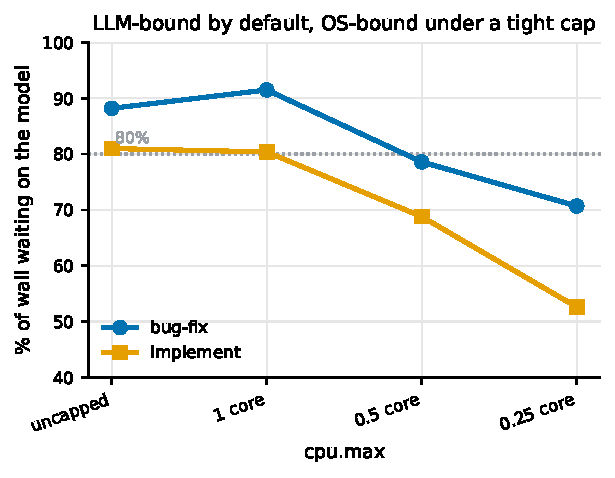
\includegraphics[width=0.85\linewidth]{fig_llmshare}
\caption{Share of wall-clock time the agent spends waiting on the model.
${\ge}80\%$ uncapped; it falls as \texttt{cpu.max} tightens and throttle
fills the wall. Medians, $n{=}5$ per cap.}
\label{fig:llm}
\end{figure}

\section{Problem 1: CPU Bandwidth Cap}
\label{sec:cpu}

\paragraph{Setup.} We cap the agent's cgroup with \texttt{cpu.max} at
unlimited, 1, 0.5, and 0.25 core, for two tasks (bug-fix, implement),
5 reps each (40 runs).

\paragraph{Result.} The agent's compute demand is fixed at roughly 4--5
CPU-seconds, whatever the cap. The cap does not reduce the work; it turns
compute into \emph{throttle wait}. Table~\ref{tab:cpu} shows both tasks:
on-CPU time is flat while throttled time and wall time climb as the cap
tightens.

\begin{table}[t]\centering\footnotesize
\setlength{\tabcolsep}{4pt}
\caption{Problem~1, medians over $n{=}5$. On-CPU demand is flat across
caps; the cap converts it into throttle wait. ``thr.'' is throttled time in
seconds and as a fraction of wall.}
\label{tab:cpu}
\begin{tabular}{@{}lrrrrr@{}}
\toprule
\texttt{cpu.max} & wall (s) & $\Delta$wall & on-CPU (s) & thr.\ (s) & thr.\ \% \\
\midrule
\multicolumn{6}{@{}l}{\textit{bug-fix}} \\
unlimited & 23.4 & --     & 4.4 & 0.0  & 0 \\
1 core    & 24.4 & $+4$\%  & 3.7 & 0.3  & 1 \\
0.5 core  & 22.4 & $-4$\%  & 3.7 & 4.4  & 20 \\
0.25 core & 28.9 & $+24$\% & 3.9 & 13.7 & 47 \\
\addlinespace
\multicolumn{6}{@{}l}{\textit{implement}} \\
unlimited & 18.7 & --     & 5.2 & 0.0  & 0 \\
1 core    & 18.7 & $+0$\%  & 5.0 & 0.5  & 2 \\
0.5 core  & 23.7 & $+27$\% & 5.2 & 6.3  & 27 \\
0.25 core & 32.7 & $+75$\% & 5.3 & 19.8 & 61 \\
\bottomrule
\end{tabular}
\end{table}

\paragraph{Interpretation.} At 1 core the agent is still LLM-bound. At
0.5 core and below, the CPU cap becomes first-order. This establishes the
regime framing used throughout: an agent is LLM-bound until a per-resource
threshold, after which the OS dominates. (Confirms hypotheses H1--H2.)












\section{Problem 2: Threads vs.\ Cores}
\label{sec:threads}

\paragraph{Setup.} The agent launches $W \in \{2,4,8,16\}$ identical
CPU-bound workers on the 4-vCPU machine with no cgroup limit, 5 reps each
(20 runs). With $W$ runnable threads on $C$ cores, queueing theory predicts
that each thread spends a fraction $(W-C)/W$ of its time
runnable-but-waiting.

\paragraph{Result.} Table~\ref{tab:threads} shows a clean dose-response.
Per-worker on-CPU time is flat, since the work is identical. The parallel
phase inflates purely from run-queue waiting. The measured wait fraction
matches the $(W{-}C)/W$ law almost exactly: at $W{=}8$, $0.93/1.87=0.497$
vs.\ a predicted $0.500$; at $W{=}16$, $2.81/3.76=0.747$ vs.\ $0.750$.
Scheduling stalls of $\ge 1$\uu{ms} jump from tens to thousands once $W>C$,
and a $\ge 10$\uu{ms} tail appears only in the over-subscribed regime.
Against the saturated ($W{=}C$) baseline, phase wall inflates by $+91\%$ at
$2\times$ and $+295\%$ at $4\times$ over-subscription.

\begin{table}[t]\centering\footnotesize
\setlength{\tabcolsep}{4pt}
\caption{Problem~2A, medians, $n{=}5$, $C{=}4$ cores. Per-worker on-CPU
time is flat; beyond $W{=}C$ the phase inflates purely from run-queue
waiting, matching $(W{-}C)/W$. Stall columns count scheduling stalls of at
least that length.}
\label{tab:threads}
\begin{tabular}{@{}rrrrrrr@{}}
\toprule
$W$ & load & phase (s) & wait & pred. & $\ge$1\,ms & $\ge$10\,ms\\
\midrule
2  & 0.5$\times$ & 0.42 & 0.00 & 0.00 & 8    & 1 \\
4  & 1$\times$   & 0.98 & 0.05 & 0.00 & 21   & 3 \\
8  & 2$\times$   & 1.87 & 0.50 & 0.50 & 2550 & 2 \\
16 & 4$\times$   & 3.87 & 0.75 & 0.75 & 5228 & 138 \\
\bottomrule
\end{tabular}
\end{table}

\paragraph{Does the harness do this to itself?} We separately asked Claude
Code to launch $N{=}4,8$ \emph{sub-agents} in parallel, each running the
same worker (6 observational runs). The harness \emph{probes the machine}
(exactly 18 \texttt{sched\_getaffinity}/\texttt{sysinfo} calls per run,
independent of $N$) and does \emph{not} over-subscribe the CPU. The
sub-agents' CPU bursts are uncontended ($\approx\!0.4$\uu{s} each,
runnable-wait ${\approx}0$, ${\sim}20$ stalls vs.\ 2550 for raw
over-subscription) and staggered across the phase. Each sub-agent is
blocked on its own LLM turn rather than fighting for a core. The contention
of Problem~2A is therefore real, but it requires \emph{explicit}
over-parallelism (e.g.\ \texttt{xargs -P}, a forced concurrency setting, or
an under-provisioned shared box). It does not come from the default
sub-agent path. (Confirms H2--H3; H1 observed.)

\section{Problem 3: Memory Cap}
\label{sec:mem}

\paragraph{Setup.} We press the agent's memory from two directions, because
the kernel's response depends on whether the pressured memory is
\emph{reclaimable}. The agent plus a 1\,GB file working set is
${\approx}1.38$\,GB. Part~A varies the soft limit \texttt{memory.high} on a
file-reading workload (20 runs). Part~B varies the hard limit
\texttt{memory.max}, first on the same file workload (12 runs) and then on a
512\,MB anonymous-allocation workload (12 runs).

\paragraph{Part A: recoverable slowdown.} With a soft cap above the working
set, the file stays cached (zero refaults, ${\approx}6.5$\uu{s}). Below it,
every pass re-reads from disk: ${\approx}1.05$ million page refaults and a
$4.7\times$ slower phase (${\approx}30$\uu{s}), see Table~\ref{tab:mem}.
The reclaim \emph{CPU} stall is tiny (${\approx}0.16$\uu{s}); the cost is
the refault \emph{I/O}. The soft cap throttles the group (8--9k
\texttt{memory.high} events) but never kills it.

\begin{table}[t]\centering\footnotesize
\setlength{\tabcolsep}{4pt}
\caption{Problem~3A (\texttt{memory.high}), medians, $n{=}5$. Agent + file
working set ${\approx}1.38$\,GB. Below it, every pass refaults from disk;
``$\times$'' is slowdown vs.\ unlimited.}
\label{tab:mem}
\begin{tabular}{@{}lrrrr@{}}
\toprule
\texttt{memory.high} & phase (s) & $\times$ & refaults & \texttt{high} ev.\\
\midrule
unlimited & 6.5  & $1.0$ & 0            & 0 \\
1536\,MB  & 6.5  & $1.0$ & 0            & 0 \\
1152\,MB  & 30.4 & $4.7$ & 1\,049\,673  & 8505 \\
768\,MB   & 30.4 & $4.7$ & 1\,049\,884  & 9296 \\
\bottomrule
\end{tabular}
\end{table}

\begin{table}[t]\centering\footnotesize
\setlength{\tabcolsep}{4pt}
\caption{Problem~3B, the OOM cliff (\texttt{memory.max} + 512\,MB anon),
$n{=}3$. Agent + workload ${\approx}762$\,MB; sharp binary threshold.}
\label{tab:cliff}
\begin{tabular}{@{}lccc@{}}
\toprule
\texttt{memory.max} & OOM-killed & task fails & verdict\\
\midrule
1024\,MB & 0/3 & 0/3 & survives \\
896\,MB  & 0/3 & 0/3 & survives \\
768\,MB  & 0/3 & 0/3 & survives \\
640\,MB  & 3/3 & 3/3 & \textbf{OOM} \\
\bottomrule
\end{tabular}
\end{table}

\paragraph{Part B, file workload: a hard cap does not always kill.} On the
\emph{file} workload, even a tight \texttt{memory.max} (down to 768\,MB)
causes \emph{no} OOM kill. Clean page cache is always reclaimable, so the
kernel reclaims it (paying the same refault cost) instead of killing. The
OOM cliff requires \emph{unreclaimable} (anonymous) memory.

\paragraph{Part B, anonymous workload: the OOM cliff.} On the 512\,MB
anonymous workload (agent + workload ${\approx}762$\,MB), the outcome is a
sharp, reproducible step (Table~\ref{tab:cliff}). A \texttt{memory.max} of
1024, 896, or 768\,MB succeeds every time (3/3), while 640\,MB fails every
time (3/3) with an OOM kill and a failed task. Notably, the OOM killer takes
the \emph{worker} (the largest anonymous consumer), not the node process.
The agent \emph{survives and reports the failed task} rather than crashing.
In short: your sandbox memory limit silently kills your tools mid-task.
(Confirms H1--H4.)

\section{Problem 4: Disk-I/O Bandwidth Cap}
\label{sec:io}

\paragraph{Setup.} We cap the cgroup's read bandwidth with \texttt{io.max}
\texttt{rbps} at unlimited, 200, 100, and 50\uu{MB/s} on a cold 1\,GB
single-read workload (caches dropped first), 5 reps each (20 runs).

\paragraph{Result.} Once the cap drops below native disk speed, phase wall
scales as $\text{bytes}/\text{rbps}$ (Table~\ref{tab:io}). The worker reads
1\,GB in 20.4\uu{s} at a 50\uu{MB/s} cap (an exact 50\uu{MB/s}) and in
10.1\uu{s} at 100\uu{MB/s}. \texttt{io.stat} confirms the same bytes moved
in every cell, so the growth is pure throttling.

\begin{table}[t]\centering\footnotesize
\setlength{\tabcolsep}{4pt}
\caption{Problem~4 (\texttt{io.max rbps}), medians, $n{=}5$. Same bytes read
in every cell (\texttt{io.stat}); a cap above the ${\approx}205$\uu{MB/s}
native speed cannot bite.}
\label{tab:io}
\begin{tabular}{@{}lrrr@{}}
\toprule
\texttt{io.max rbps} & phase (s) & $\times$ & effective\\
\midrule
unlimited    & 5.98 & $1.0$ & ${\approx}205$\uu{MB/s} \\
200\uu{MB/s} & 5.98 & $1.0$ & ${\approx}205$\uu{MB/s} \\
100\uu{MB/s} & 10.1 & $1.7$ & ${\approx}100$\uu{MB/s} \\
50\uu{MB/s}  & 20.4 & $3.4$ & ${\approx}50$\uu{MB/s} \\
\bottomrule
\end{tabular}
\end{table}

\paragraph{Caveat.} The 200\uu{MB/s} cap has no effect because the VM's
disk only reaches ${\approx}205$\uu{MB/s}. A cap above the device's real
bandwidth cannot throttle. On faster storage, a lower cap is needed to see
the effect. (Confirms H2--H3.)

\section{Cross-Agent Consistency}
\label{sec:consistency}

To test that these effects are properties of agentic workloads rather than
of one harness, we repeated all four problems with a second, unrelated
agent: Codex CLI (a Rust/tokio binary) driving a different model
(\texttt{gpt-6-luna}) through a different API (OpenRouter)---130 runs at
parity with the Claude campaign. The scheduling, memory-reclaim and I/O
results are \emph{identical} to within noise
(Table~\ref{tab:consistency}), because those workloads are fixed worker
processes the agent merely launches. The CPU-cap and LLM-share results show
the same trends on both agents: both are ${\ge}80\%$ LLM-bound uncapped and
both shed that share under tighter caps.

The one difference is instructive. The OOM cliff sits at \emph{agent
RSS $+$ workload}, so the leaner Rust harness (Codex, small RSS) survives a
640\,MB cap that kills the Node harness (Claude, ${\approx}250$\,MB RSS).
The cliff is real for both; its location simply tracks the agent's own
footprint---a leaner harness buys headroom.

\begin{table}[t]\centering\small
\caption{Claude vs.\ Codex, medians. Scheduling/memory/I/O match to within
noise; the CPU cap shows the same trend (Codex is leaner on CPU and slower
per turn, so its walls are larger).}
\label{tab:consistency}
\begin{tabular}{llrr}
\toprule
problem & metric & Claude & Codex\\
\midrule
threads $W{=}16$ & phase (s)        & 3.9 & 3.8 \\
threads $W{=}16$ & runnable/wkr (s) & 2.8 & 2.8 \\
mem.\ 768M       & phase (s)        & 30.4 & 30.4 \\
io 50\uu{MB/s}   & phase (s)        & 20.4 & 20.4 \\
CPU 0.25 core    & throttle (s)     & 19.8 & 18.7 \\
CPU 0.25 core    & model-\% wall    & 53 & 62 \\
\bottomrule
\end{tabular}
\end{table}

\section{Discussion}

\paragraph{It is not just the LLM.} The agent is ${\approx}84\%$ LLM-bound on
an adequate machine, so blaming the model is understandable. But across four
independent resources a single mis-set container limit adds $1.7$--$4.7\times$
wall time or kills the agent's tools outright---far above the ``even 5\%
would be significant'' bar, at sandbox sizes common in practice
(fractional-CPU CI runners, tight memory pods).

\paragraph{Two shapes of harm.} Bandwidth limits (CPU, disk, and soft
memory) cause \emph{recoverable slowdown}; a hard limit on an unreclaimable
resource (anonymous memory, no swap) causes \emph{failure}. CPU
over-subscription is a third, \emph{self-inflicted} slowdown. A fault
catalogue for agents should distinguish these, because they call for
different remedies (right-size vs.\ add swap/headroom vs.\ bound
concurrency).

\paragraph{Configuration is the villain, not the harness.} Because a
well-behaved harness checks cores and avoids CPU over-subscription
(Section~\ref{sec:threads}), the danger is concentrated in the limits a
platform imposes---exactly the parameter nobody profiles when an agent
``feels slow.''

\paragraph{Everything is kernel-visible.} Each effect appears in both the
LTTng trace and the cgroup's own counters, and the two agree. This makes the
method a reusable recipe for a larger fault catalogue rather than a set of
one-off anecdotes.

\paragraph{Limitations.} The main uncontrolled input is LLM
nondeterminism, mitigated by fixed prompts, byte-identical repos, randomized
order, and medians; each result is reproducible to $<\!1\%$ across reps and
cross-validated against an independent kernel counter. The findings are
tied to a single machine shape: no swap (so anonymous pressure OOMs rather
than swaps), an SMT topology (effective zero-contention core count 2--4),
and one disk speed (which sets where the I/O knee falls). Tasks are small;
larger agent sessions with more local work would shift each threshold toward
milder caps, strengthening the effect rather than weakening it.

\section{Conclusion}

An AI coding agent is ${\approx}84\%$ LLM-bound on an adequate machine, but a
single mis-configured container limit---on CPU, cores, memory, or disk
I/O---pushes it into an OS-bound regime where the operating system, not the
model, is the bottleneck, adding up to $4.7\times$ latency or killing the
agent's tools. We characterized four such configuration-level problems with
kernel traces, located each threshold, validated every measurement against
the kernel's own accounting, and reproduced the effects on a second,
unrelated agent. The practical message is blunt: when an agent feels slow,
profile the sandbox, not only the model.

\paragraph{Artifacts.} Collection and analysis scripts, per-run metadata and
provenance (environment snapshot, campaign logs, manifests), and the full
results are available in the project repository under
\texttt{Blueprint/latency/}.

\end{document}
